\documentclass[a4paper,
fontsize=11pt,
%headings=small,
oneside,
numbers=noperiodatend,
parskip=half-,
bibliography=totoc,
final
]{scrartcl}

\usepackage[babel]{csquotes}
\usepackage{synttree}
\usepackage{graphicx}
\setkeys{Gin}{width=.4\textwidth} %default pics size

\graphicspath{{./plots/}}
\usepackage[ngerman]{babel}
\usepackage[T1]{fontenc}
%\usepackage{amsmath}
\usepackage[utf8x]{inputenc}
\usepackage [hyphens]{url}
\usepackage{booktabs} 
\usepackage[left=2.4cm,right=2.4cm,top=2.3cm,bottom=2cm,includeheadfoot]{geometry}
\usepackage[labelformat=empty]{caption} % option 'labelformat=empty]' to surpress adding "Abbildung 1:" or "Figure 1" before each caption / use parameter '\captionsetup{labelformat=empty}' instead to change this for just one caption
\usepackage{eurosym}
\usepackage{multirow}
\usepackage[ngerman]{varioref}
\setcapindent{1em}
\renewcommand{\labelitemi}{--}
\usepackage{paralist}
\usepackage{pdfpages}
\usepackage{lscape}
\usepackage{float}
\usepackage{acronym}
\usepackage{eurosym}
\usepackage{longtable,lscape}
\usepackage{mathpazo}
\usepackage[normalem]{ulem} %emphasize weiterhin kursiv
\usepackage[flushmargin,ragged]{footmisc} % left align footnote
\usepackage{ccicons} 
\setcapindent{0pt} % no indentation in captions

%%%% fancy LIBREAS URL color 
\usepackage{xcolor}
\definecolor{libreas}{RGB}{112,0,0}

\usepackage{listings}

\urlstyle{same}  % don't use monospace font for urls

\usepackage[fleqn]{amsmath}

%adjust fontsize for part

\usepackage{sectsty}
\partfont{\large}

%Das BibTeX-Zeichen mit \BibTeX setzen:
\def\symbol#1{\char #1\relax}
\def\bsl{{\tt\symbol{'134}}}
\def\BibTeX{{\rm B\kern-.05em{\sc i\kern-.025em b}\kern-.08em
    T\kern-.1667em\lower.7ex\hbox{E}\kern-.125emX}}

\usepackage{fancyhdr}
\fancyhf{}
\pagestyle{fancyplain}
\fancyhead[R]{\thepage}

% make sure bookmarks are created eventough sections are not numbered!
% uncommend if sections are numbered (bookmarks created by default)
\makeatletter
\renewcommand\@seccntformat[1]{}
\makeatother

% typo setup
\clubpenalty = 10000
\widowpenalty = 10000
\displaywidowpenalty = 10000

\usepackage{hyperxmp}
\usepackage[colorlinks, linkcolor=black,citecolor=black, urlcolor=libreas,
breaklinks= true,bookmarks=true,bookmarksopen=true]{hyperref}
\usepackage{breakurl}

%meta
%meta

\fancyhead[L]{L. Freyberg\\ %author
LIBREAS. Library Ideas, 43 (2023). % journal, issue, volume.
\href{https://doi.org/10.18452/...}{\color{black}https://doi.org/10.18452/...}
{}} % doi 
\fancyhead[R]{\thepage} %page number
\fancyfoot[L] {\ccLogo \ccAttribution\ \href{https://creativecommons.org/licenses/by/4.0/}{\color{black}Creative Commons BY 4.0}}  %licence
\fancyfoot[R] {ISSN: 1860-7950}

\title{\LARGE{Eine soziologische Perspektive auf Smart Libraries }}% title
\author{Linda Freyberg} % author

\setcounter{page}{1}

\hypersetup{%
      pdftitle={Eine soziologische Perspektive auf Smart Libraries},
      pdfauthor={Linda Freyberg},
      pdfcopyright={CC BY 4.0 International},
      pdfsubject={LIBREAS. Library Ideas, 43 (2023).},
      pdfkeywords={Smart Libraries, Raumkonzept, Soziologie Radovan Richta, Deleuze, Guattari},
      pdflicenseurl={https://creativecommons.org/licenses/by/4.0/},
      pdfurl={https://doi.org/10.18452/...},
      pdfdoi={10.18452/...},
      pdflang={de},
      pdfmetalang={de}
     }



\date{}
\begin{document}

\maketitle
\thispagestyle{fancyplain} 

%abstracts
\begin{abstract}
\noindent
\textbf{Kurzfassung}: In diesem Beitrag wird eine Definition des
Konzeptes der Smart Libraries gegeben und vor dem Hintergrund
technologischer Entwicklungen im Spannungsfeld zwischen Kontinuität und
Wandel eingeordnet. Dabei werden (technik-) philosophische und
soziologische Theorien eingebunden, die größere Fragen aufwerfen und zur
weiteren Lektüre einladen.

\begin{center}\rule{0.5\linewidth}{0.5pt}\end{center}
\end{abstract}

%body
\emph{Dieser Text basiert in Teilen auf:}

\emph{Freyberg, Linda (2018): Smart Libraries -- buzz word or tautology?
In: Elephant in the Lab, 2. Juli 2018,
\url{https://doi.org/10.5281/zenodo.1302988}.}

\hypertarget{einleitung}{%
\section{Einleitung}\label{einleitung}}

Der Begriff \enquote{Smart Library} wurde in den letzten Jahren als Teil
eines ganzheitlichen \enquote{Smart City}-Konzepts vermehrt verwendet,
um eine Vision der Bibliothek der Zukunft zu zeichnen. Dieses Konzept
adressiert die Integration digitaler Prozesse und informationeller
Partizipation in die urbane öffentliche Infrastruktur und entwirft einen
erstrebenswerten Zustand, in dem Städte \enquote{smarter}, das heißt
effizienter organisiert und ressourcenschonender, flexibler,
nachhaltiger, grüner, inklusiver und sozialer werden. Bibliotheken sind
als öffentliche Einrichtungen Teil dieses Entwicklungs- und
Optimierungsprozesses. Ob es sich dabei um \enquote{glatte oder gekerbte
Räume}\footnote{Deleuze, Gilles; Guattari, Félix (1980): 1440 -- Das
  Glatte und das Gekerbte. In: Dünne, Jörg; Günzel, Stephan (Hrsg.):
  Raumtheorie. Grundlagentexte aus Philosophie und Kulturwissenschaften;
  Suhrkamp Taschenbuch Verlag; Frankfurt am Main, 2006; S. 434.}
handelt, sie sich also geordnet und stabil manifestiert (bzw.
\enquote{gekerbt}) zeigen oder variabel sind und sich stetig im Fluss
befinden (bzw. \enquote{glatt}), ist zu diskutieren. Eine gelungene
technikphilosophische Lesart der beiden Raumkonzepte von Deleuze und
Guattari entwickelt Kaja Tulatz: \enquote{Im gekerbten Raum wird
{[}...{]} auf Kontingenzreduktion gezielt, während im glatten Raum nach
Kontingenzerweiterung gestrebt wird.}\footnote{Tulatz, Kaja:
  Technikinduzierte Räume bei Deleuze und Guattari. XXII. Deutscher
  Kongress für Philosophie, 11. - 15. September 2011.
  \url{https://doi.org/10.5282/ubm/epub.12570}. S.1.} Speziell in Bezug
auf smarte Bibliotheken wäre die Frage, ob \enquote{smart} etwas
Absolutes ist und \enquote{keine Steigerungsform} besitzt, wie Moritz
Mutter zunächst feststellt, oder es darum geht, \enquote{Probleme in
Gelegenheiten zu transformieren}\footnote{Mutter, Moritz (2019): Klug
  werden: Zur Semantik des Begriffs \enquote{smart}. In: Freyberg,
  Linda; Wolf, Sabine (Hrsg.): Smart Libraries. Konzepte, Methoden und
  Strategien. Wiesbaden: b.i.t Verlag, S. 18.} und damit immer im Fluss
zu bleiben. Auch zu hinterfragen ist, ob die Entwicklung von
Bibliotheken einer Logik des Fortschritts, im Sinne einer ständigen
Weiterentwicklung und Verbesserung vergleichbar mit Francis Bacons
Konzept des \enquote{progressus scientiarium}\footnote{Renn, Jürgen
  (2022): Die Evolution des Wissens. Eine Neubestimmung der Wissenschaft
  für das Anthropozän. Berlin: Suhrkamp Verlag. S.\,50\,f.} unterworfen
ist oder sich gerade durch eine Konstanz auszeichnet.

Festzuhalten ist, dass mit dem Zustand der ständigen Veränderung nicht
alle zufrieden sind und die Vision einer Smart City nicht unumstritten
ist (siehe das Graffito aus Berlin-Kreuzberg in Abb. 1).

\begin{figure}
\centering
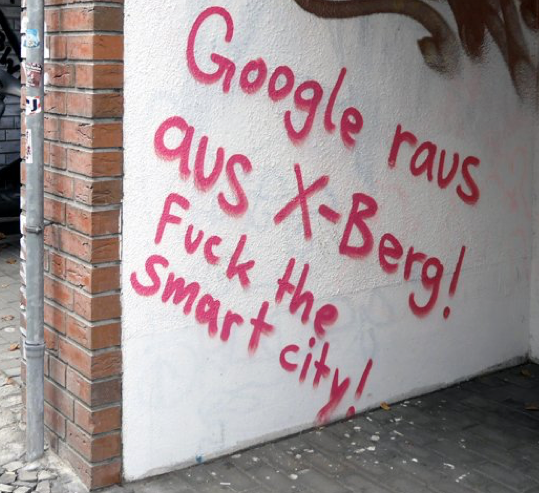
\includegraphics[width=0.5\textwidth]{img/Fig.3_Fuck_Smart_City.png}
\caption{Abb. 1: Ben Kaden/Twitter 23.10.2017, bearbeitet}
\end{figure}

Für Bibliotheken, ob smart oder nicht, stellt sich die Frage, was es
bedeutet, Teil dieser Entwicklung zu sein. Was ist ihre Rolle und wie
sollten sie handeln? Und was bedeutet es für eine Bibliothek, überhaupt
\enquote{smart} zu sein?

\hypertarget{konzept-smart-library}{%
\section{Konzept Smart Library}\label{konzept-smart-library}}

Obwohl bereits internationale Pilotprojekte\footnote{Siehe zum Beispiel
  \url{https://www.aakb.dk/smartlibrary}.} in Bibliotheken und
Konferenzen\footnote{Siehe Smart Libraries for Tomorrow (2016):
  \url{https://www.las.org.sg/wp/lft/}.} zu diesem Thema stattgefunden
haben, gibt es keine umfassende Definition einer \enquote{Smart
Library}.

Der Schwerpunkt von \enquote{smart} im aktuellen Sprachgebrauch liegt
auf dem sinnvollen Einsatz von Technologie (siehe \enquote{smart phone})
und ragt semantisch in den Bereich der Automatisierung (zum Beispiel
\enquote{smart home}), Alltagskoordination (zum Beispiel \enquote{smart
mobility}) und der künstlichen Intelligenz (oft im Zusammenhang mit
\enquote{smart data}).

Es ist klar, dass Bibliotheken nicht nur durch den Einsatz von
Technologien smart werden, sondern sich Modernisierung auf viele Aspekte
wie den physischen Raum oder digitale Angebote bezieht und innerhalb der
Institutionen auf Personal- und Führungsebene und außerhalb der
Einrichtungen durch Kooperationen und partizipative Prozesse im
Idealfall durch ganzheitliche Konzepte verankert sind.

Eine aktuelle, die genannten Aspekte umfassende, Definition einer Smart
Library von Sabine Wolf lautet:

\begin{quote}
\enquote{Eine Smart Library zeichnet sich durch einen hohen
Anwendungsgrad moderner (Informations-)Technologien aus. Sie ist offen
für Kooperationen aller Art und unterstützt proaktiv eine
Personalentwicklung im Sinn einer zukunftsfähigen Bibliothek. Diese drei
Kennzeichen sind eingebettet in eine agile Bibliotheksentwicklung und
werden ergänzt durch eine Partizipation von Nutzerinnen und Nutzern.
Ausgestattet mit einer Informationsinfrastruktur und einer
entsprechenden Möblierung bietet sie diesen einen Aufenthaltsqualität,
die das Lernen unterstützt und die Bibliothek als Treffpunkt
etabliert.}\footnote{Wolf, Sabine (2019): Definition einer Smart Library
  und Erläuterung der Smart Map. Ein State-of-the-Art-Ansatz. In:
  Freyberg, Linda; Wolf, Sabine (Hrsg.): Smart Libraries. Konzepte,
  Methoden und Strategien. Wiesbaden: b.i.t Verlag. S. 21.}
\end{quote}

Auch wenn \enquote{Smart Library} oft als modisches Schlagwort verwendet
wird, stellt der Begriff offensichtlich mehr dar als nur ein Etikett
oder eine glatte, blinkende Oberfläche. Generell sollte der Einsatz von
Technologien und innovativen Veränderungen also in ein umfassendes
strategisches Gesamtkonzept eingebettet sein, das den lokalen
Anforderungen der Mitarbeiter*innen und der Nutzenden entspricht.

Denn natürlich funktioniert nicht jede Strategie für jede Institution,
und daher ist einer der grundlegenden Ansätze in diesem Zusammenhang
eine gründliche Untersuchung und Bewertung der Entwicklungsziele. So ist
die Beobachtung von Trends, die beispielsweise im jährlichen
Gartner\textquotesingle s Hype Cycle oder dem IFLA-Trendreport
veröffentlicht werden, eine wichtige Aufgabe für die Bibliotheken.
Weitere Quellen sind der ALA TechSource Blog und deren Website
\enquote{Library of the Future} sowie Konferenzen und Messen. Leider
existiert der einzige periodische Bericht mit Fokus auf Bibliotheken,
der NMC-Report, nicht mehr, aber Alternativen und Ideen für einen neuen
Bibliothekstrendbericht wurden in der Community bereits
diskutiert\footnote{Siehe Schuldt, Karsten (2018): Wie könnte ein
  besserer Zukunftsreport für Bibliotheken aussehen?
  \url{https://bildungundgutesleben.wordpress.com/2018/01/22/wie-koennte-ein-besserer-zukunftsreport-fuer-bibliotheken-aussehen/}.}.

\hypertarget{kontext-soziologie-der-bibliothek}{%
\section{Kontext Soziologie der
Bibliothek}\label{kontext-soziologie-der-bibliothek}}

Ein wesentlicher Aspekt dieses Konzeptes und der damit verbundenen
Strategien ist, dass es sich um eine Art Antwort auf Herausforderungen
und scheinbar um eine Lösung für Probleme handelt. Das heißt, zunächst
einmal muss es eine Frage oder ein Infragestellen geben, zum Beispiel:
Ist die Idee einer Bibliothek noch zeitgemäß? Haben Bibliotheken in der
heutigen Informationsgesellschaft noch eine Daseinsberechtigung?
Bibliotheken auf der ganzen Welt sind mit diesen Fragen konfrontiert,
unter anderem auch, weil diese regelmäßig an sie herangetragen werden.
Der Erfolg der (meisten) Bibliotheken ist wirtschaftlich nicht messbar,
auch weil diese Einrichtungen nicht nach kapitalistischen Kriterien
konzipiert sind und sich somit dieser Logik entziehen. Bibliotheken sind
(für die Nutzenden mehr oder weniger) kostenlos und für jedermann und
jedefrau offen, was eher einem kommunistischen oder gemeinnützigen
Prinzip folgt. Universitäts- oder Forschungsbibliotheken sind Teil eines
akademischen Umfelds als Anbieterinnen von wissenschaftlicher Literatur
und Vermittlerinnen wissenschaftlicher Kommunikation. Daher sind sie von
größeren Wissenschaftsinstitutionen abhängig, aber auch durch diese
abgesichert und in ihrer Funktion legitimiert. Öffentliche Bibliotheken
hingegen sind von den Kommunen abhängig und mit lokaler Politik
konfrontiert. Ihre räumliche Einbindung in die unmittelbare
Nachbarschaft und somit die Produktion von Attraktivität als Ort bieten
die Grundlage strategischer Bemühungen. Das Etablieren als sogenannter
dritter Ort wurde in den letzten Jahren hinreichend und erschöpfend
diskutiert. Kurz gesagt geht es dabei., assoziativ angelehnt an Ray
Oldenburg\footnote{Siehe Oldenburg, Ray (1999): The Great Good Place --
  cafés, coffee shops. bookstores, bars, hair salons and other hangouts
  at the heart of the community. New York : Marlowe and Company.}, um
das Schaffen eines ergänzenden Lebensbereichs mit hoher
Aufenthaltsqualität neben dem zu Hause und dem Arbeitsplatz. In der
Praxis bedeutet dies oftmals, dass Sofas aufgestellt, Loungebereiche
eingerichtet und Cafés in Bibliotheken integriert werden.

Übergeordnet gewinnen auch Konzepte wie Bürgerbeteiligung bzw. Community
Engagement, Open Government oder Citizen Science zunehmend, vor allem
für Öffentliche Bibliotheken, an Relevanz.

Ein Grund, warum sowohl Öffentliche als auch Wissenschaftliche
Bibliotheken zunehmend in Frage gestellt werden, sind natürlich die
Möglichkeiten des World Wide Web, also die Wahrnehmung eines schier
endlosen Zugangs zu massenhaft digital \enquote{frei} verfügbaren
Informationen zu allen erdenklichen Themen in allen möglichen
Medienformen, scheinbar ohne von einer vermittelnden Institution
abhängig zu sein. Die Herausforderung für Bibliotheken liegt heute
darin, an dieser Entwicklung teilzuhaben und das Digitale zu integrieren
und mitzudenken, ohne ihre Grundfunktionen und ihre Gemeinnützigkeit
aufzugeben.

Zugleich lässt sich fragen, ob die Grundidee einer Bibliothek nicht an
sich schon ziemlich smart ist? Bibliotheken sind als Ort der Bildung,
als Sammlerinnen und Anbieterinnen von Informationen und Wissen
etabliert und genießen ein gewisses Vertrauen, wenn es darum geht,
gesicherte Informationen zu vermitteln. Und genau diese Funktionen
werden auch in Zukunft noch nötig, wenn nicht sogar existentiell, sein.
Gerade vor dem Hintergrund von Phänomenen wie der Informationsflut und
der Desinformationen, braucht es eine Institutionen ohne eigene
(kommerzielle) Interessen, die bei der Recherche und bei der
Identifikation relevanter und auch glaubwürdiger Informationen
unterstützt und im Idealfall die transparente, kritische und
reflektierte Einordnung von Quellen fördert. Bekanntlich sind einerseits
das Kuratieren, traditionell durch Bestandsaufbau, im Digitalen stärker
durch die Organisation von Zugang sowie anderseits die
Kompetenzvermittlung für die Nutzung der Inhalte und das Verständnis von
Informationsprozessen aktuelle Leitaufgaben der Bibliotheken.

Um nun auch explizit den Bogen zur Soziologie zu spannen: Der
tschechische Soziologe und Philosoph Radovan Richta beschäftigte sich in
den 1960er-Jahren mit technischen Umwälzungen und den gesellschaftlichen
Konsequenzen dieser. Sein bekanntestes Werk ist wohl der sogenannte
\enquote{Richta-Report}\footnote{Richter, Radovan und Kollektiv (Hrsg.)
  (1968): Richta-Report. Politische Ökonomie des 20. Jahrhunderts. Die
  Auswirkungen der technisch-wissenschaftlichen Revolution auf die
  Produktionsverhältnisse. Marxistische Bibliothek, Text 10. Frankfurt
  a.M.: makol Verlag.}, den er gemeinsam mit über 60 Autor*innen
erarbeitete. Dabei berücksichtigte er bereits mathematische Maschinen
(Computer), die seiner Prognose nach stark an Relevanz zunehmen
werden.\footnote{Richter, S. 34.}

Der Begriff \enquote{smart} bezieht sich vor allem auf die Effizienz
durch den Einsatz von Technologien und auf die Automatisierung von
Prozessen zur Erleichterung des Arbeits- und Alltagsumfeldes. Richta
spricht in diesem Kontext von einer Verdrängung der menschlichen
Tätigkeit in \enquote{vorproduktive Stufen} wie \enquote{die
Vorbereitung der Technik}\footnote{Ebenda.}. So wie \enquote{Smart
Homes} versprechen, das Leben zu erleichtern und freizumachen von der
trivialen Bedienung von einzelnen Geräten, hält auch in Bibliotheken die
Automatisierung Einzug. So übernehmen beispielsweise Bücherroboter
weniger anspruchsvolle Aufgaben wie die Rückgabe, die Lagerung oder auch
die Bereitstellung von Medien. Während sich viele Bibliothekar*innen von
diesen tristen Routinen entlastet fühlen und froh sind, sich auf
anspruchsvollere Tätigkeiten konzentrieren zu können, evoziert dies auch
die Angst im Zuge der Automatisierung, überflüssig oder ersetzbar zu
werden. Wenn die Mitarbeitenden nicht mehr für Routinetätigkeit benötigt
werden, ist die betriebswirtschaftliche Schlussfolgerung nicht in jedem
Fall, sie für anspruchsvollere Tätigkeiten einzusetzen. Nicht selten
spart man sie einfach komplett ein. Dies ist eine der Entwicklungen, mit
denen sich Bibliotheken auseinandersetzen müssen. Wir wissen aktuell
nicht, inwieweit und wie schnell Künstliche Intelligenz (KI) in die
intellektuelle Arbeit hinein wirken wird. Die KI-fizierung als
Fortsetzung der Automatisierung wird aber mit Sicherheit früher oder
später auch die Arbeit in den Bibliotheken verändern.

Zusammenfassend lässt sich sagen, dass Bibliotheken als
nicht-kommerzielle Anbieterinnen und Sammlerinnen vielleicht schon immer
\enquote{smart} waren, denn neben der Bereitstellung von Informationen
mussten Bibliotheken stets den Fortschritt managen und sich in einem
permanenten Prozess erneuern, was den Begriff der \enquote{Smart
Library} vielleicht sogar etwas tautologisch macht. Die Hauptfunktionen
von Bibliotheken bleiben weitestgehend gleich. Aber durch die enorme
Zunahme von digital verfügbaren Informationen und deren Relevanz sowie
durch neue Präsentations- und Zugangsformen muss stetig über neue Wege
der Vermittlung, neue Dienstleistungen und neue Umgebungen nachgedacht
werden.

\hypertarget{referenzen}{%
\section{Referenzen}\label{referenzen}}

Deleuze, Gilles; Guattari, Félix (1980): 1440 -- Das Glatte und das
Gekerbte. In: Dünne, Jörg; Günzel, Stephan (Hrsg.): Raumtheorie.
Grundlagentexte aus Philosophie und Kulturwissenschaften; Suhrkamp
Taschenbuch Verlag; Frankfurt am Main, 2006.

Mutter, Moritz (2019): Klug werden: Zur Semantik des Begriffs
\enquote{smart}. In: Freyberg, Linda; Wolf, Sabine (Hrsg.): Smart
Libraries. Konzepte, Methoden und Strategien. Wiesbaden: b.i.t Verlag.
S. 17--19.

Oldenburg, Ray (1999): The Great Good Place -- cafés, coffee shops.
bookstores, bars, hair salons and other hangouts at the heart of the
community. New York : Marlowe and Company.

Richta, Radovan und Kollektiv (Hrsg.) (1968): Richta-Report. Politische
Ökonomie des 20. Jahrhunderts. Die Auswirkungen der
technisch-wissenschaftlichen Revolution auf die Produktionsverhältnisse.
Marxistische Bibliothek, Text 10. Frankfurt a.M.: makol Verlag.

Renn, Jürgen (2022): Die Evolution des Wissens. Eine Neubestimmung der
Wissenschaft für das Anthropozän. Berlin: Suhrkamp Verlag.

Schuldt, Karsten (2018): Wie könnte ein besserer Zukunftsreport für
Bibliotheken aussehen?
\href{https://bildungundgutesleben.wordpress.com/2018/01/22/wie-koennte-ein-besserer-zukunftsreport-fuer-bibliotheken-aussehen/}{https://bildungundgutesleben.wordpress.com/2018/01/22/wie-koennte-ein-besserer-zukunfts-report-fuer-bibliotheken-aussehen/}.

Tulatz, Kaja (2011): Technikinduzierte Räume bei Deleuze und Guattari.
XXII. Deutscher Kongress für Philosophie, 11. - 15. September 2011.
\url{https://doi.org/10.5282/ubm/epub.12570}.

Wolf, Sabine (2019): Definition einer Smart Library und Erläuterung der
Smart Map. Ein State-of-the-Art-Ansatz. In: Freyberg, Linda; Wolf,
Sabine (Hrsg.): Smart Libraries. Konzepte, Methoden und Strategien.
Wiesbaden: b.i.t Verlag, S. 21--26,
\url{https://www.b-i-t-online.de/daten/bit_Innovativ_76_Freyberg_Wolf_Leseprobe.pdf}.

%autor

\begin{center}\rule{0.5\linewidth}{0.5pt}\end{center}

\textbf{Dr. Linda Freyberg} ist promovierte Kulturwissenschaftlerin und arbeitet als Wissenschaftlerin an der BBF | Bibliothek für Bildungsgeschichtliche Forschung des DIPF | Leibniz-Institut für Bildungsforschung und Bildungsinformation in Berlin. Sie ist Redakteurin der LIBREAS. Library Ideas. ORCID: \url{https://orcid.org/0000-0002-4620-7571}

\end{document}